
\documentclass[UTF8]{beamer}
%\usepackage{subfigure}
\usepackage{url}   % 网页链接
\usepackage{subcaption}
%\usepackage[space,space,hyperref]{ctex}
%\usepackage{ctex} %可以改成中文版
\captionsetup{font={small}}
\usetheme{Warsaw}
\author{Tong Wu}
\title{Partially coherent ptychography}
%\institute{Sun yat-sen University, China}
\begin{document}
\frame{\titlepage}
%\tableofcontents


\begin{frame}[c]\frametitle{Coherent model}


\begin{equation}
\label{basic}
f_{j}=\left|\mathcal{F}\left( \mathcal{S}_{j} u  \circ \omega \right)\right|^{2} 
\end{equation}

In a discrete setting, $u \in \mathbb{C}^{n}$ is a 2D image with $\sqrt{n} \times \sqrt{n}$ pixels, $\omega \in \mathbb{C}^{\bar{m}}$ is a localized 2D probe with $\sqrt{\bar{m}} \times \sqrt{\bar{m}}$ pixels.

$f_{j} \in \mathbb{R}_{+}^{\bar{m}}(\forall 0 \leq j \leq J-1)$ is a stack of phaseless measurements. Here $|\cdot|$ represents the element-wise absolute value of a vector, o denotes the elementwise multiplication, and $\mathcal{F}$ denotes the normalized 2 dimensional discrete Fourier transform. Each $\mathcal{S}_{j} \in \mathbb{R}^{\bar{m} \times n}$ is a binary matrix that crops a region $j$ of size $\bar{m}$ from the image $u$.


\end{frame}

\begin{frame}[c]\frametitle{Partially coherent model: a general one}
\framesubtitle{Thibault, Pierre, and Andreas Menzel. "Reconstructing state mixtures from diffraction measurements." Nature 494.7435 (2013): 68-71.}



\structure{Blind ptychography model + quantum state tomography\footnote{\url{https://homepage.univie.ac.at/reinhold.bertlmann/pdfs/T2_Skript_Ch_9corr.pdf} Many symbols in quantum mechanics are included here.}.}

Phobe $w$ is assumed to be in mixed state to represent partially coherent effect.

\begin{equation}
\label{model:sep} 
\begin{aligned}
&\mbox{Find } u, r \mbox{ othogonal $w_k$   }s.t. \\
&f_{p c, j}=\sum_{k=1}^r \left|\mathcal{F}\left( \mathcal{S}_{j} u \circ \left(\omega_k\right) \right)\right|^{2}  
\end{aligned}
\end{equation}


\end{frame}

\begin{frame} \frametitle{Connection to a particular model}

Continuous setting:

\begin{equation}
f_{p c, j}(q) = \int\left|\mathcal{F}_{x \rightarrow q}\left(\mathcal{S}_{j} u(x) \omega(x-y)\right)\right|^{2} \kappa(y) \mathrm{d} y
\end{equation}

Discrete setting:

\begin{equation}
f_{p c, j}=\sum_{i} \kappa_{i}\left|\mathcal{F}\left( \mathcal{S}_{j} u \circ \left(\mathcal{T}_{i} \omega\right) \right)\right|^{2}
\label{model:target}
\end{equation}

 We put the $\kappa_{i}$ inside:
\begin{equation}
f_{p c, j}=\sum_{i} \left|\mathcal{F}\left( \mathcal{S}_{j} u \circ \left( \sqrt{\kappa_{i}}\mathcal{T}_{i} \omega\right) \right)\right|^{2}
=
\sum_{i} \left|\mathcal{F}\left( \mathcal{S}_{j} u \circ \left( \hat{\omega}_i\right) \right)\right|^{2}
\end{equation}
Multiple modes $\hat{w}_i$ are produced by shifted $w$. Then we can construct density matrix and use truncated SVD to get a low-rank approximation. Then it is exactly \eqref{model:sep}
$$
\rho = \sum_i \hat{w}_i \hat{w}_i^* \approx \sum_{k=1}^{r} w_k w_k^* 
$$

\end{frame}




\begin{frame} \frametitle{Algorithm design}

Generally find a low-rank matrix $\rho$ based on \eqref{model:sep}, which has
special structures based on particular models like \eqref{model:target}

Two possible ways:

\begin{enumerate}

\item \structure{Transfer existing algorithms}:  

related to Low-rank Matrix Recovery

\item \structure{Exploit new structure}:

Rank-1 Matrix + vibration kernel $\kappa$ $\rightarrow$ matrix $\rho$

The rank-1 matrix comes from the main mode (Bessel).

Why approximated low-rank?

Why special patterns for modes decomposed from $\rho$? 
\end{enumerate}





\end{frame}

\begin{frame} \frametitle{Example: Guassian $\kappa$ (15 15)}
\begin{figure}[H]
\centering
%\caption{}
\begin{subfigure}{1\textwidth}
    \centering
    % include first image
    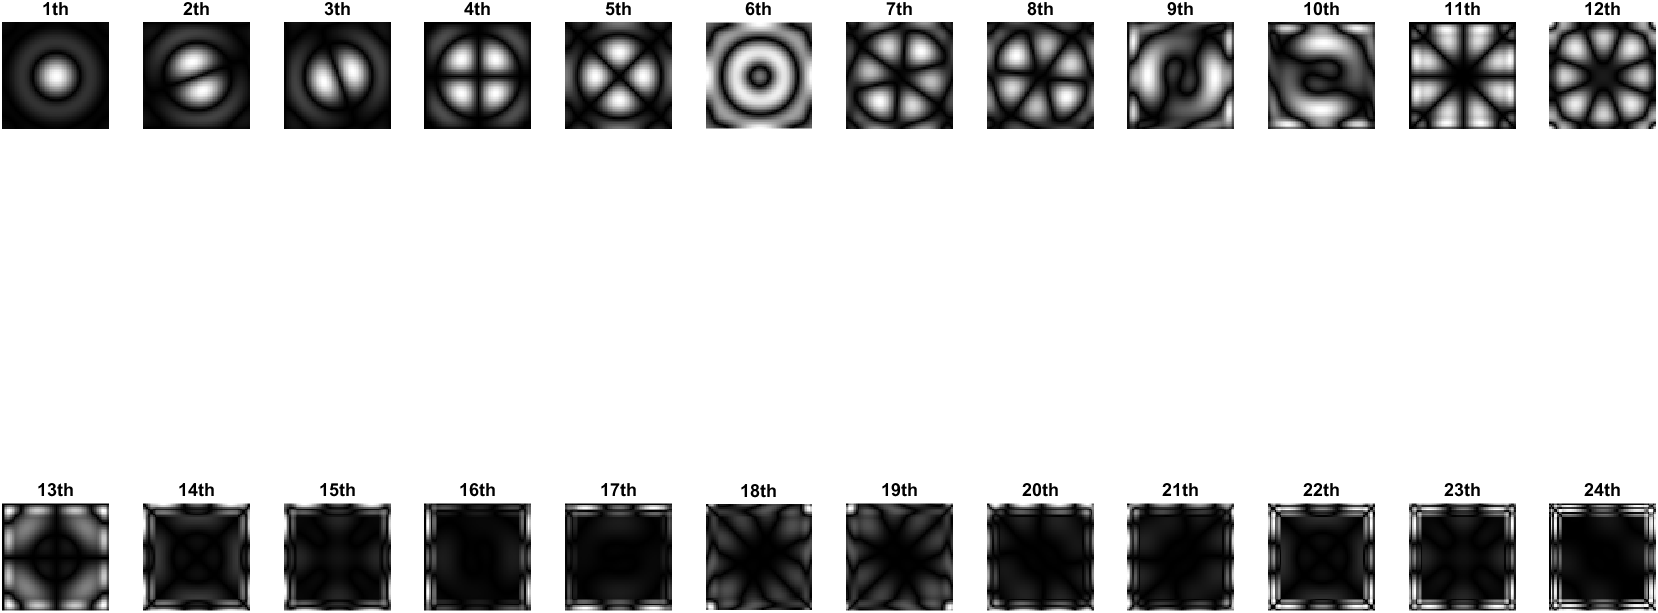
\includegraphics[width=0.9\linewidth]{../figures/ex_gu15_15.png}  
   %\caption{Ideal modes}
    \label{fig:modes_u}
 \end{subfigure}
 \begin{subfigure}{1\textwidth}
    \centering
    % include second image
    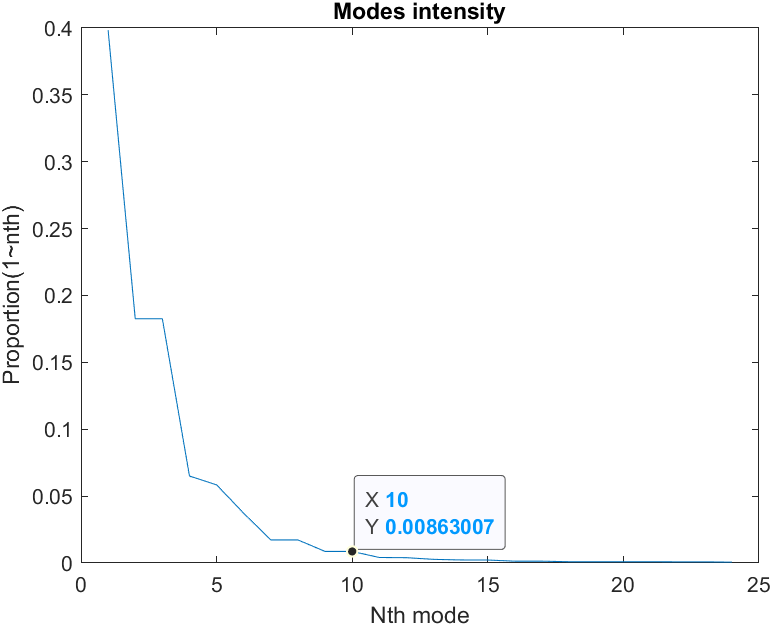
\includegraphics[width=.5\linewidth]{../figures/ex_gu15_15_s.png}  
    %\caption{Put your sub-caption here}
    %\caption{Singular value distribution}
    \label{fig:modes_u_phaze}
 \end{subfigure}
 
    \label{fig:modes_images}

 \end{figure}
\end{frame}


\begin{frame} \frametitle{Example: Retangular $\kappa$ (20 20)}
\begin{figure}[H]
\centering
\begin{subfigure}{1\textwidth}
    \centering
    % include first image
    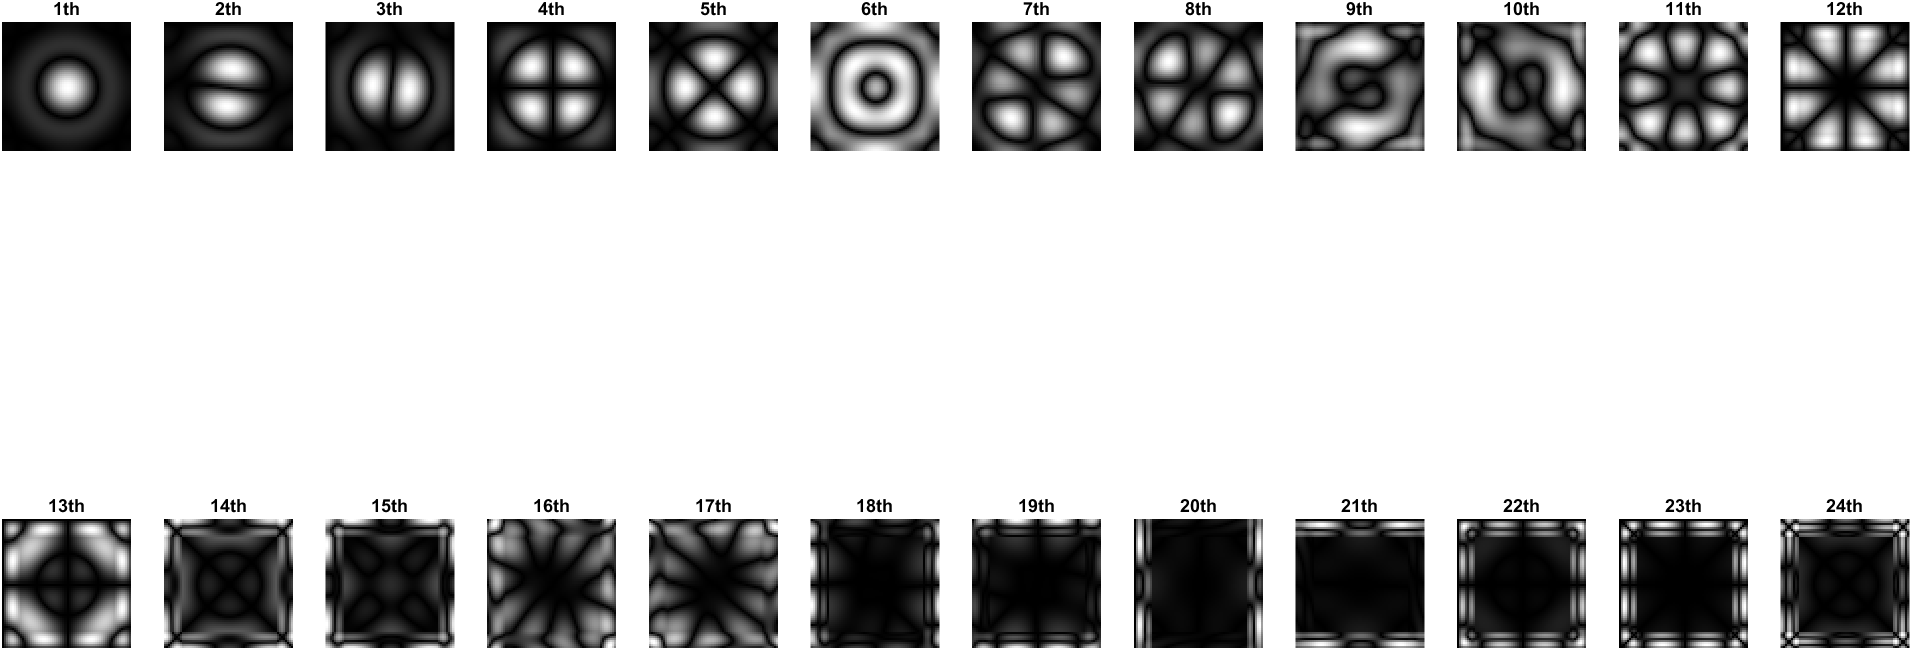
\includegraphics[width=0.9\linewidth]{../figures/ex_ave20.png}  
   %\caption{Ideal modes}
    \label{fig:modes_u}
 \end{subfigure}
 \begin{subfigure}{1\textwidth}
    \centering
    % include second image
    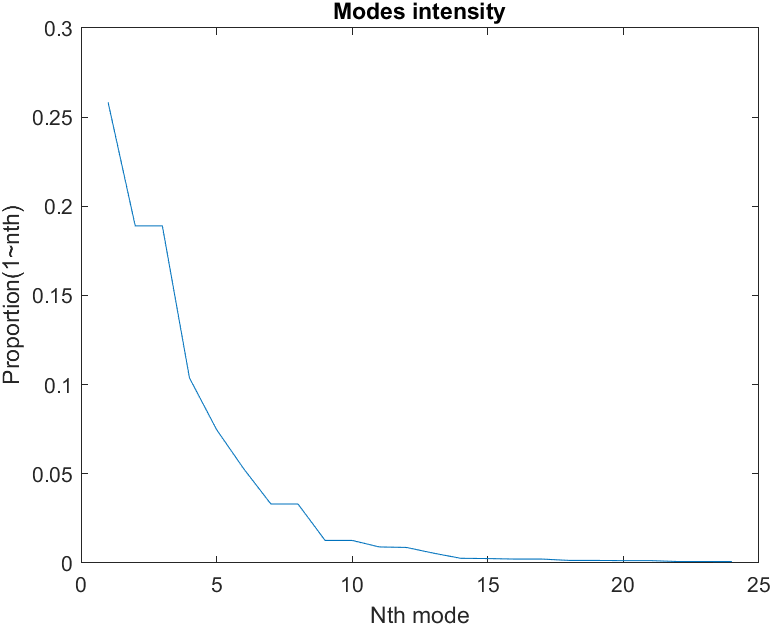
\includegraphics[width=.5\linewidth]{../figures/ex_ave20_s.png}  
    %\caption{Put your sub-caption here}
    %\caption{Singular value distribution}
    \label{fig:modes_u_phaze}
 \end{subfigure}
 \end{figure}
\end{frame}

\begin{frame} \frametitle{Example: Guassian $\kappa$ (4 0)}
\begin{figure}[H]
\centering
\begin{subfigure}{1\textwidth}
    \centering
    % include first image
    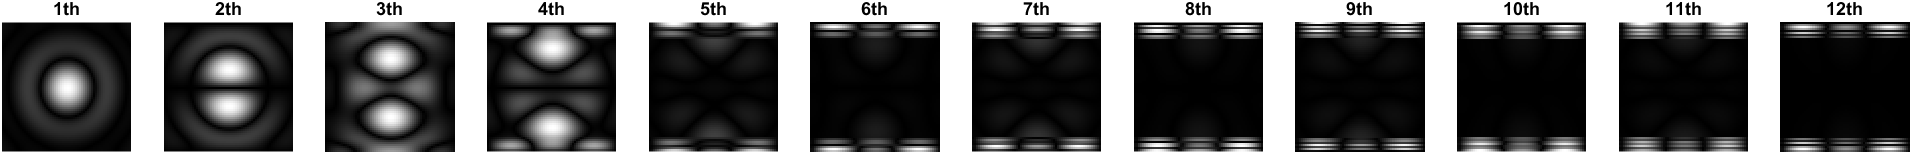
\includegraphics[width=0.9\linewidth]{../figures/ex_gu4_0.png}  
   %\caption{Ideal modes}
    \label{fig:modes_u}
 \end{subfigure}
 \begin{subfigure}{1\textwidth}
    \centering
    % include second image
    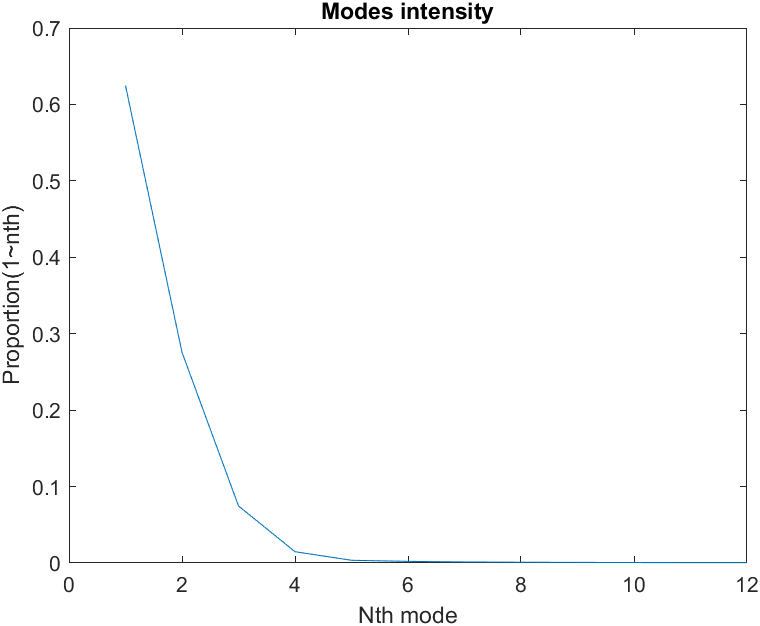
\includegraphics[width=.5\linewidth]{../figures/ex_gu4_0_s.png}  
    %\caption{Put your sub-caption here}
    %\caption{Singular value distribution}
    \label{fig:modes_u_phaze}
 \end{subfigure}
 \end{figure}
\end{frame}

\begin{frame} \frametitle{Example: Motion $\kappa$ (len=20,theta=45)}
\begin{figure}[H]
\centering
\begin{subfigure}{1\textwidth}
    \centering
    % include first image
    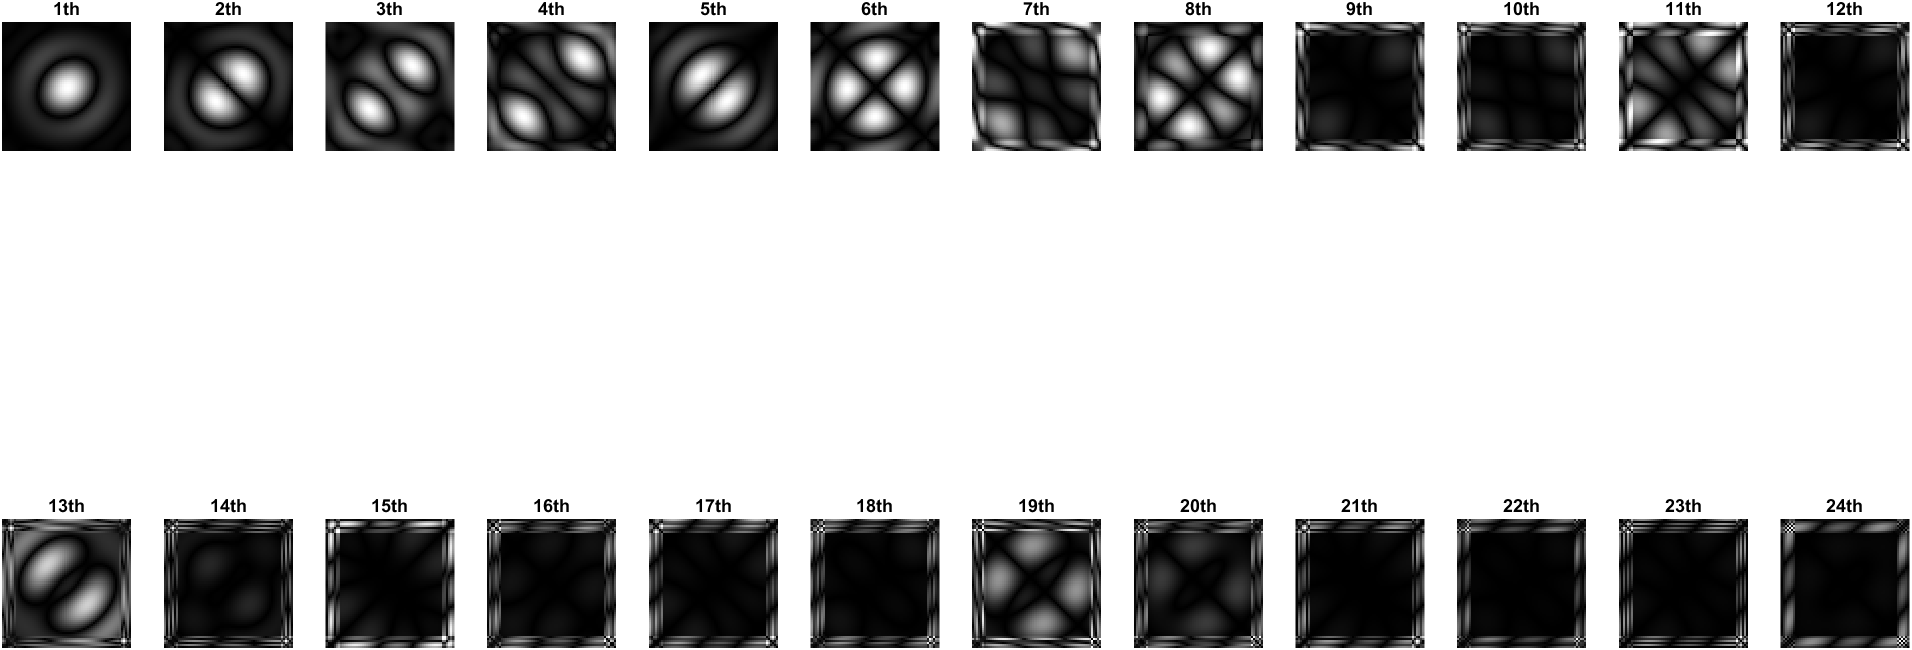
\includegraphics[width=0.9\linewidth]{../figures/ex_motion.png}  
   %\caption{Ideal modes}
    \label{fig:modes_u}
 \end{subfigure}
 \begin{subfigure}{1\textwidth}
    \centering
    % include second image
    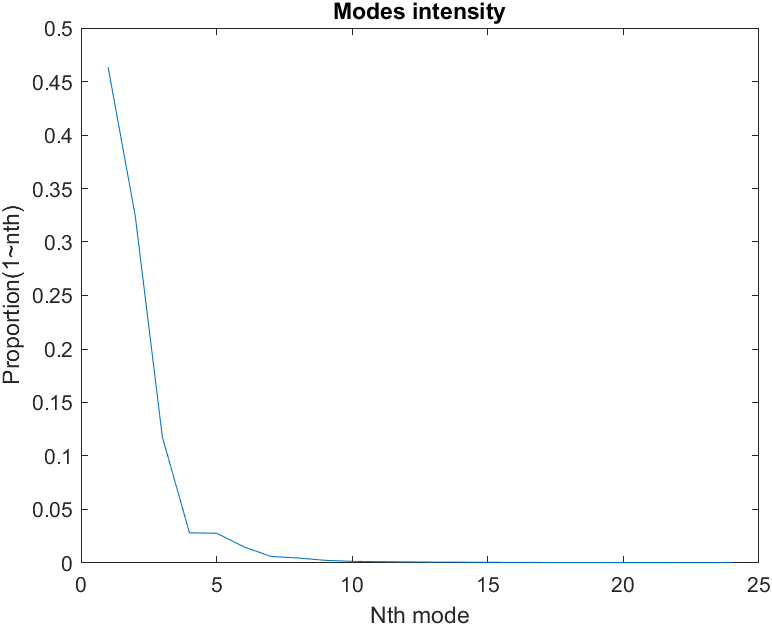
\includegraphics[width=.5\linewidth]{../figures/ex_motion_s.png}  
    %\caption{Put your sub-caption here}
    %\caption{Singular value distribution}
    \label{fig:modes_u_phaze}
 \end{subfigure}
 \end{figure}
\end{frame}

\begin{frame} \frametitle{More about Bessel}
\begin{figure}[H]
\centering

    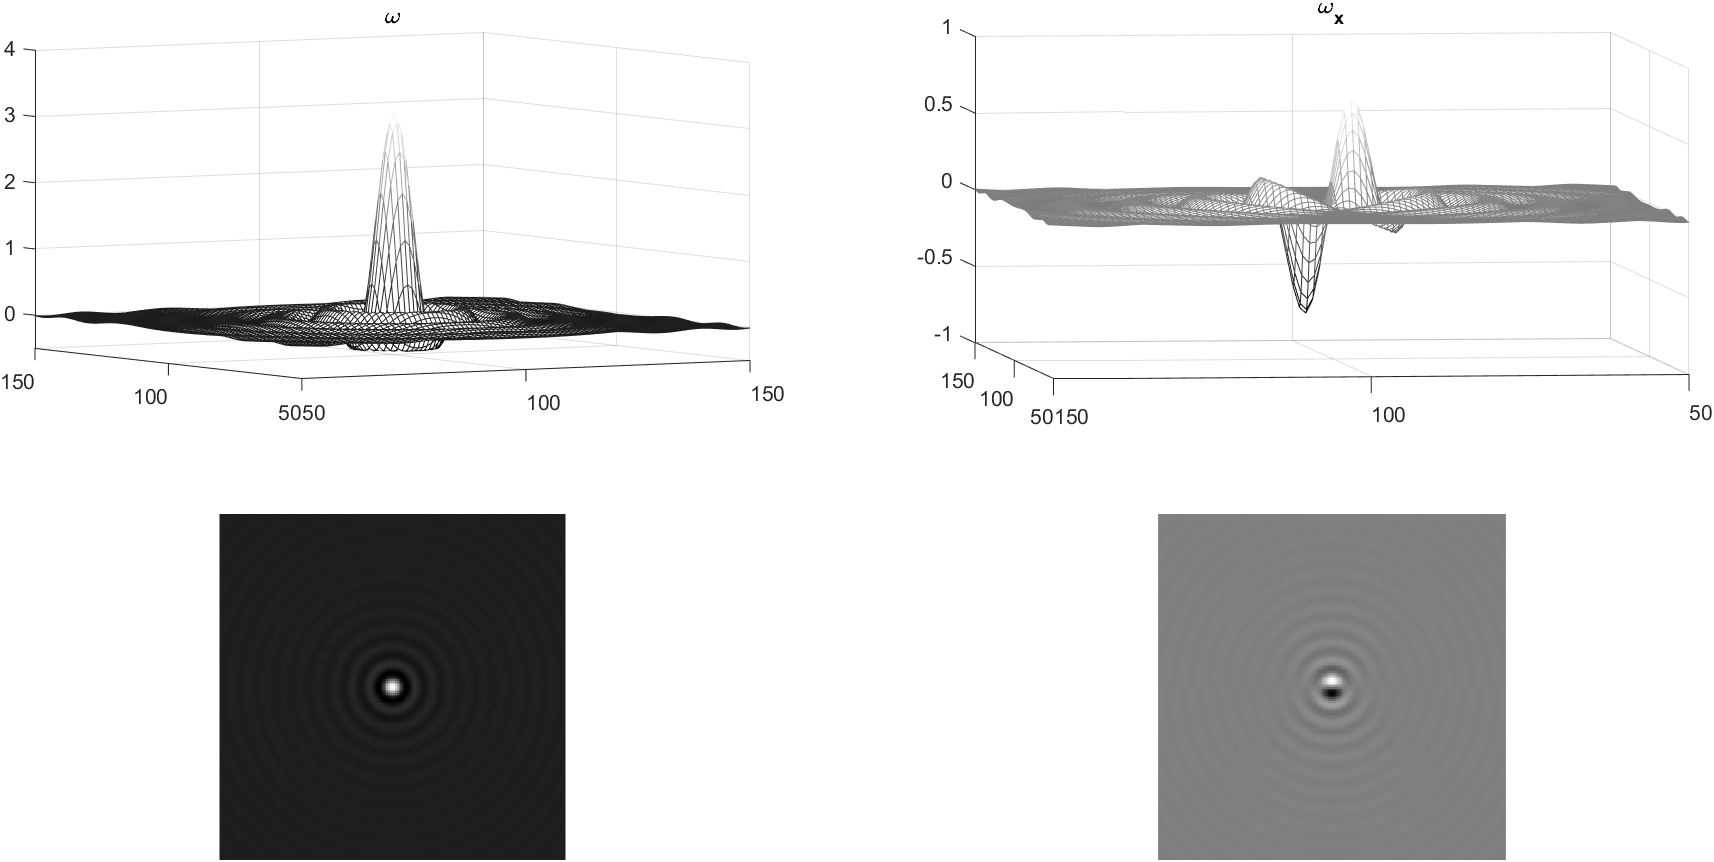
\includegraphics[width=0.9\linewidth]{../figures/bessel_cp.png}  
   
\end{figure}
\end{frame}

%\begin{frame} \frametitle{}
%\centering
%
%\end{frame}

\end{document}
